\documentclass[11pt]{article}
\usepackage[margin=1in]{geometry}
\usepackage{amsmath, amssymb}
\usepackage{graphicx}

\begin{document}

\textbf{DSC 210, Fall 2026 --- Homework 1} \hfill Nicholas Wendt (200478549)

%%%%%%%%%%%%%%%%%%%%%%%%%%%%%%%%%%%%%%%%%%%%%%%%%%%%%%%%%%%%%%%%%%%%%%%%
\section*{Question 1: Property of triangular matrices (20 points)}

Given $U_1$ and $U_2$ are two upper triangular matrices of size $n\times n$, prove that $U_1U_2$ is also an upper triangular matrix. Further, prove by induction that multiplication of $m\,(m>2)$ upper triangular matrices ($U_1, U_2, \dots, U_m$) is also an upper triangular matrix.

\textbf{Solution:}
\bigskip

Since both $U_1$ and $U_2$ are upper triangular matrices that means entries $a_{ij}=0$ for $i>j$
in $U_1$ and entries $b_{ij}=0$ for $i>j$ in $U_2$.\\
Let matrix $C=U_1U_2$. We want to show that entries $c_{ij} = 0$ when $i>j$.\\
The element
$$
c_{ij} = \sum_{k=1}^na_{ik}b_{kj}=a_{i1}b_{1j}+a_{i2}b_{2j}+\cdots+a_{in}b_{nj}
$$
To show that every term in this sum is 0, we look at 2 cases.\\
\textbf{Case 1:} Let $k<i$ , then element $a_{ik}=0$\\
\textbf{Case 2:} Let $k \geq i$ , then $k \geq i > j$ , so $k > j$. Then element $b_{kj}=0$\\
So $\forall k\ , \ a_{ik}b_{kj}=0 $

\bigskip

\noindent Therefore $c_{ij} = 0$ for $i>j$ making $C$ an upper triangular matrix.

\bigskip

\noindent\textbf{Inductive step:} Assume $P_m=U_1U_2 \cdots U_m$ is an upper triangular matrix. \\
Let $U_{m+1}$ be an upper triangular $n\times n$ matrix. Since
matrix multiplication is associative,

$$
P_{m+1} = U_1U_2\cdots U_mU_{m+1} = (U_1U_2\cdots U_m)\,U_{m+1} = P_m\,U_{m+1}.
$$

\noindent By the inductive hypothesis, $P_m$ is upper triangular, and $U_{m+1}$ is upper triangular by
definition. By the base case, the product of two upper triangular matrices is upper triangular.

\medskip

\noindent So $P_mU_{m+1}$ is upper triangular. Therefore $P_{m+1}$ is upper triangular.

\bigskip

\noindent\textbf{Conclusion:} By induction, the product $U_1U_2\cdots U_m$ of upper triangular matrices is an upper triangular matrix for all $m \geq 2$. $\blacksquare$

%%%%%%%%%%%%%%%%%%%%%%%%%%%%%%%%%%%%%%%%%%%%%%%%%%%%%%%%%%%%%%%%%%%%%%%%
\newpage
\section*{Question 2: Matrix operations (20 points)}

Let $\mathbf{B}$ be a $4\times 4$ matrix to which we apply the following 7 operations sequentially and get a final matrix $\mathbf{D}$:
\begin{enumerate}
    \item[(i)] triple column 2,
    \item[(ii)] halve row 4,
    \item[(iii)] add row 2 to row 1,
    \item[(iv)] interchange columns 1 and 3,
    \item[(v)] subtract row 3 from each of the other rows,
    \item[(vi)] replace column 4 by column 2,
    \item[(vii)] delete column 1 (so that the column dimension is reduced by 1).
\end{enumerate}
\begin{enumerate}
    \item[(a)] Express each operation (i) to (vii) as a matrix and the final matrix $\mathbf{D}$ as a product of 8 matrices. (10 points)
    \item[(b)] Write the final result again as a product of $\mathbf{ABC}$, i.e.\ write matrix $\mathbf{D} = \mathbf{ABC}$ and find $\mathbf{A},\mathbf{C}$. (5 points)
    \item[(c)] Write Python code to verify your answers in parts a and b. Show the answers and code. (5 points) Let
    \[
    \mathbf{B} = \begin{bmatrix}
        2 & 1 & 0 & 3\\
        0 & 1 & 2 & -1\\
        1 & 0 & 2 & 1\\
        0 & 1 & 1 & 2
    \end{bmatrix}
    \]
    Hint: You can use NumPy for matrix operations.
\end{enumerate}

\textbf{Solution:}

\textbf{(a)}

\bigskip

First let's write out the individual operations in matrix form.\\
Note: row operations must be multiplied on the left of B while column operations are multiplied on the right.
$$
(i)=\begin{bmatrix}
    1 & 0&0&0\\
    0&3&0&0\\
    0&0&1&0\\
    0&0&0&1
\end{bmatrix},
(ii) = \begin{bmatrix}
1&0&0&0\\
0&1&0&0\\
0&0&1&0\\
0&0&0&\frac12
\end{bmatrix},
(iii)=\begin{bmatrix}
1&1&0&0\\
0&1&0&0\\
0&0&1&0\\
0&0&0&1
\end{bmatrix},
(iv)=\begin{bmatrix}
0&0&1&0\\
0&1&0&0\\
1&0&0&0\\
0&0&0&1
\end{bmatrix}
$$
$$
(v)=\begin{bmatrix}
1&0&-1&0\\
0&1&-1&0\\
0&0&1&0\\
0&0&-1&1
\end{bmatrix},
(vi)=\begin{bmatrix}
1&0&0&0\\
0&1&0&1\\
0&0&1&0\\
0&0&0&0
\end{bmatrix},
(vii)=\begin{bmatrix}
0&0&0\\
1&0&0\\
0&1&0\\
0&0&1
\end{bmatrix}
$$
Now define matrix $D$:
$$
D=(v)(iii)(ii)B(i)(iv)(vi)(vii)
$$

\textbf{(b)}
Let $A$ be the product of row operations and let $C$ be the product of column operations.
$$
A=(v)(iii)(ii)=\begin{bmatrix}
1&0&-1&0\\
0&1&-1&0\\
0&0&1&0\\
0&0&-1&1
\end{bmatrix}
\begin{bmatrix}
1&1&0&0\\
0&1&0&0\\
0&0&1&0\\
0&0&0&1
\end{bmatrix}
\begin{bmatrix}
1&0&0&0\\
0&1&0&0\\
0&0&1&0\\
0&0&0&\frac12
\end{bmatrix}
$$
Multiplying right to left we get
$$
A=\begin{bmatrix}
1&0&-1&0\\
0&1&-1&0\\
0&0&1&0\\
0&0&-1&1
\end{bmatrix}
\begin{bmatrix}
1&1&0&0\\
0&1&0&0\\
0&0&1&0\\
0&0&0&\frac12
\end{bmatrix}
=
\begin{bmatrix}
1&1&-1&0\\
0&1&-1&0\\
0&0&1&0\\
0&0&-1&\frac12
\end{bmatrix}
$$
Calculating $C$
$$
C=(i)(iv)(vi)(vii)=
\begin{bmatrix}
    1 & 0&0&0\\
    0&3&0&0\\
    0&0&1&0\\
    0&0&0&1
\end{bmatrix}
\begin{bmatrix}
0&0&1&0\\
0&1&0&0\\
1&0&0&0\\
0&0&0&1
\end{bmatrix}
\begin{bmatrix}
1&0&0&0\\
0&1&0&1\\
0&0&1&0\\
0&0&0&0
\end{bmatrix}
\begin{bmatrix}
0&0&0\\
1&0&0\\
0&1&0\\
0&0&1
\end{bmatrix}
$$
$$
=\begin{bmatrix}
    1 & 0&0&0\\
    0&3&0&0\\
    0&0&1&0\\
    0&0&0&1
\end{bmatrix}
\begin{bmatrix}
0&0&1&0\\
0&1&0&0\\
1&0&0&0\\
0&0&0&1
\end{bmatrix}
\begin{bmatrix}
0&0&0\\
1&0&1\\
0&1&0\\
0&0&0
\end{bmatrix}
$$
$$
=\begin{bmatrix}
    1 & 0&0&0\\
    0&3&0&0\\
    0&0&1&0\\
    0&0&0&1
\end{bmatrix}
\begin{bmatrix}
0&1&0\\
1&0&1\\
0&0&0\\
0&0&0
\end{bmatrix}
$$
$$
C=\begin{bmatrix}
0&1&0\\
3&0&3\\
0&0&0\\
0&0&0
\end{bmatrix}
$$
Now we can write matrix $D$ as the product of 3 matrices.
$$D=ABC=
\begin{bmatrix}
1&1&-1&0\\
0&1&-1&0\\
0&0&1&0\\
0&0&-1&\frac12
\end{bmatrix}
\begin{bmatrix}
        2 & 1 & 0 & 3\\
        0 & 1 & 2 & -1\\
        1 & 0 & 2 & 1\\
        0 & 1 & 1 & 2
    \end{bmatrix}
\begin{bmatrix}
0&1&0\\
3&0&3\\
0&0&0\\
0&0&0
\end{bmatrix}
$$



\textbf{(c)}
\begin{verbatim}
import numpy as np
B = np.array([[2,1,0,3],[0,1,2,-1],[1,0,2,1],[0,1,1,2]])

i = np.array([[1,0,0,0],[0,3,0,0],[0,0,1,0],[0,0,0,1]])
ii = np.array([[1,0,0,0],[0,1,0,0],[0,0,1,0],[0,0,0,0.5]])
iii = np.array([[1,1,0,0],[0,1,0,0],[0,0,1,0],[0,0,0,1]])
iv = np.array([[0,0,1,0],[0,1,0,0],[1,0,0,0],[0,0,0,1]])
v = np.array([[1,0,-1,0],[0,1,-1,0],[0,0,1,0],[0,0,-1,1]])
vi = np.array([[1,0,0,0],[0,1,0,1],[0,0,1,0],[0,0,0,0]])
vii = np.array([[0,0,0],[1,0,0],[0,1,0],[0,0,1]])

# part a
D = v @ iii @ ii @ B @ i @ iv @ vi @ vii
print("D =\n", D)

# part b
A = v @ iii @ ii
C = i @ iv @ vi @ vii
print("A =\n", A)
print("C =\n", C)
print("ABC =\n", A @ B @ C)
\end{verbatim}
We see that
$$
D=\begin{bmatrix}
6&1&6\\
3&-1&3\\
0&1&0\\
\frac32&-1&\frac32
\end{bmatrix}
$$

%%%%%%%%%%%%%%%%%%%%%%%%%%%%%%%%%%%%%%%%%%%%%%%%%%%%%%%%%%%%%%%%%%%%%%%%
\newpage
\section*{Question 3: Matrix properties (20 points)}

Prove that if a matrix $\mathbf{A}$ is triangular (upper or lower) then $\mathbf{A}^{-1}$ is also triangular. Further, use the result to show that if $\mathbf{A}$ is both triangular and orthogonal, then it is diagonal.

\textbf{Solution:}\\
Let $A$ be an invertible upper triangular matrix. \\
Since $\det A$ is the product of the diagonal entries and $\det A \neq 0$, every diagonal entry $a_{ii}$ is nonzero.
\medskip

\noindent The $j$-th column, $\mathbf{x}$, of $A^{-1}$ satisfies $A\mathbf{x} = \mathbf{e}_j$ since $AA^{-1}=I$ where $e_j$ is the $j$-th column of $I$. 
Solve this system by back substitution, starting from the bottom row.
\smallskip

Every entry of $\mathbf{e}_j$ below row $j$ is $0$.

Let $\mathbf{x}$ be the $j$-th column of $A^{-1}$, so that $A\mathbf{x} = \mathbf{e}_j$. Then each entry $x_k$ of $\mathbf{x}$ is the $(k,j)$ entry of $A^{-1}$, and we want to show $x_k = 0$ for every $k > j$.
\bigskip

Assume $j < n$. Every entry of $\mathbf{e}_j$ below row $j$ is $0$. The last row of the system $A\mathbf{x} = \mathbf{e}_j$ reads $a_{nn}x_n = 0$
Since $a_{nn} \neq 0$, $x_n = 0$.
Thus every column of $A^{-1}$ has zeros below the diagonal, so $A^{-1}$ is upper triangular.

If $A$ is lower triangular, then $A^T$ is upper triangular, so $(A^T)^{-1} = (A^{-1})^T$ is upper triangular. 
Therefore $A^{-1}$ is lower triangular. $\blacksquare$

\bigskip

\textbf{Part 2.} Suppose $A$ is upper triangular and orthogonal; the lower triangular case is the same. Orthogonality gives $A^TA = I$, so $A^{-1} = A^T$.

By Part 1, $A^{-1}$ is upper triangular. But $A^T$ is lower triangular, because it is the transpose of an upper triangular matrix. Since $A^{-1} = A^T$, this matrix is both upper and lower triangular, so it is diagonal.

Hence $A^T$ is diagonal, and therefore $A$ is diagonal. $\blacksquare$
\bigskip


%%%%%%%%%%%%%%%%%%%%%%%%%%%%%%%%%%%%%%%%%%%%%%%%%%%%%%%%%%%%%%%%%%%%%%%%
\newpage
\section*{Question 4: $p$-norm inequalities (20 points)}

Let $\mathbf{x}$ be a real $m$-vector. The vector $p$-norms $\lVert \mathbf{x} \rVert_{p}$ are related by various inequalities, often involving the dimension of the vector, i.e.\ $m$. For parts (a) and (b), prove the inequality and give an example of a nonzero vector $\mathbf{x}$ for which \textit{equality} is satisfied.
\begin{enumerate}
    \item[(a)] $\lVert \mathbf{x} \rVert_2 \le \lVert \mathbf{x} \rVert_1$. (7 points)
    \item[(b)] $\lVert \mathbf{x} \rVert_2 \le \sqrt{m} \cdot \lVert \mathbf{x} \rVert_\infty$. (7 points)
    \item[(c)] Plot a 2D contour of $\lVert \mathbf{x} \rVert_1 = 1$; on the same chart also highlight regions where $\lVert \mathbf{x}\rVert_2 < 1$, $\lVert \mathbf{x}\rVert_2 = 1$ and $\lVert \mathbf{x}\rVert_2 > 1$. Describe where the contour intersects $\lVert \mathbf{x} \rVert_2 = 1$. (6 points)
\end{enumerate}

\textbf{Solution:}

\textbf{(a)}
Start by taking the square of the 1-norm.
$$
\Vert \textbf{x} \Vert_1^2=(|x_1|+|x_2|+ \cdots + |x_m|)^2=\sum_{i=1}^m|x_i|^2+\sum_{i\neq j}|x_i||x_j|
$$
The first sum is exactly $\Vert \textbf{x} \Vert_2^2$ and every $|x_i||x_j| \geq 0$. So we get
$$
\Vert \textbf{x} \Vert_1^2 \geq \Vert \textbf{x} \Vert_2^2
$$
Both norms are nonnegative so we can safely take the square root without the inequality changing.
Therefore
$$
\lVert \mathbf{x} \rVert_2 \le \lVert \mathbf{x} \rVert_1 \quad \blacksquare
$$
Example: One nonzero entry with all other entries being 0.\\
Let
$$
\textbf{x}=\begin{bmatrix}
    0\\-7\\0\\\vdots\\ 0
\end{bmatrix}
$$
Then
$$
\lVert \mathbf{x} \rVert_2=\sqrt{0^2-7^2+0^2+\cdots+0^2}=7
$$
and
$$
\lVert \mathbf{x} \rVert_1=|0|+|-7|+|0|+\cdots+|0|=7
$$

\textbf{(b)}
Recall that $\Vert \textbf{x} \Vert_{\infty}=max(|x_1|,|x_2|,...,|x_m|)$.\\
Then each entry satisfies $|x_i|\leq \Vert \textbf{x} \Vert_{\infty}$.
And then each $x_i^2\leq \Vert \textbf{x} \Vert_{\infty}^2$.
There are $m\ x_i's$ so we sum both sides of the inequality.
$$
x_1^2+x_2^2+\cdots +x_m^2\leq \Vert \textbf{x} \Vert_{\infty}^2 +\Vert \textbf{x} \Vert_{\infty}^2+\cdots +
\Vert \textbf{x} \Vert_{\infty}^2=m \Vert \textbf{x} \Vert_{\infty}^2
$$
We see the left side
$$
x_1^2+x_2^2+\cdots +x_m^2=\Vert \textbf{x} \Vert_2^2
$$
So we get
$$
\Vert \textbf{x} \Vert_2^2 \leq m \Vert \textbf{x} \Vert_{\infty}^2
$$
Since both sides are nonnegative, taking the square root gives
$$
\Vert \textbf{x} \Vert_2 \leq \sqrt{m} \Vert \textbf{x} \Vert_{\infty} \quad \blacksquare
$$
Example: All elements in $\textbf{x}$ are nonzero and have the same absolute value.\\
Let
$$
\textbf{x}=\begin{bmatrix}
    2\\2\\ \vdots\\2
\end{bmatrix}
$$
Then
$$
\Vert \textbf{x} \Vert_2=\sqrt{2^2+2^2+\cdots + 2^2}=\sqrt{4+4+\cdots +4}=\sqrt{4m}=2\sqrt{m}
$$
and 
$$
\Vert \textbf{x} \Vert_{\infty}=max(2,2,...,2)=2 \rightarrow 2\sqrt{m}
$$
\bigskip
\textbf{(c)}
\begin{figure}[h]
  \centering
  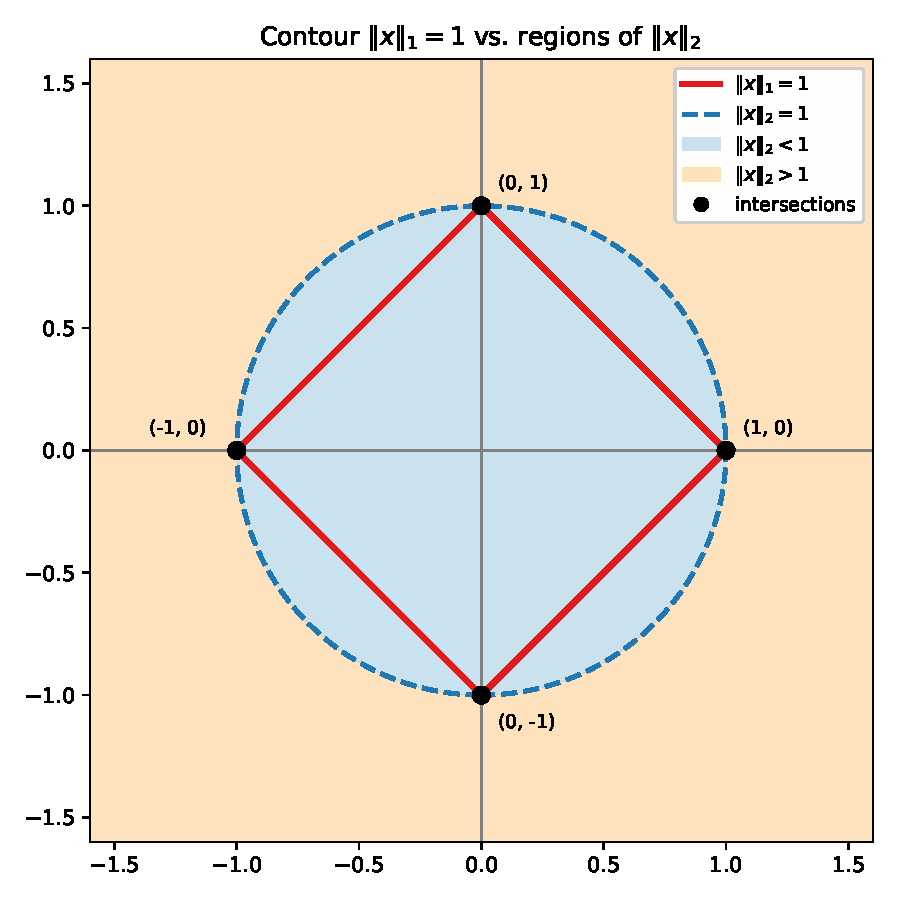
\includegraphics[width=0.6\linewidth]{l1_l2_contour.pdf}
\end{figure}

The contour $\|x\|_1=1$ intersects $\|x\|_2=1$ only at the four points
$(\pm1,0)$ and $(0,\pm1)$. 

% Save your plot as plot.png in this folder, then uncomment the next line:
% \includegraphics[width=0.6\textwidth]{plot.png}

%%%%%%%%%%%%%%%%%%%%%%%%%%%%%%%%%%%%%%%%%%%%%%%%%%%%%%%%%%%%%%%%%%%%%%%%
\newpage
\section*{Question 5: Basic vector operations (20 points)}

Given two 3-dimensional vectors $\mathbf{a}, \mathbf{b}$, and three matrices $\mathbf{A} \in \mathbb{R}^{3 \times 2}$, $\mathbf{B} \in \mathbb{R}^{2 \times 3}$, $\mathbf{C} \in \mathbb{R}^{3 \times 2}$, and scalars $\beta_1, \beta_2$ with the values below:
\begin{gather*}
    \mathbf{a} = \begin{bmatrix} 1 \\ 5 \\ 9 \end{bmatrix},\quad
    \mathbf{b} = \begin{bmatrix} 2 \\ 6 \\ 10 \end{bmatrix},\quad
    \mathbf{A} = \begin{bmatrix} 1 & 4 \\ 2 & 5 \\ 3 & 6 \end{bmatrix},\quad
    \mathbf{B} = \begin{bmatrix} 7 & 8 & 9 \\ 10 & 11 & 12 \end{bmatrix},\quad
    \mathbf{C} = \begin{bmatrix} 1 & 0 \\ 0 & 0 \\ 0 & 1 \end{bmatrix},\quad
    \beta_1 = 2,\ \beta_2 = 3
\end{gather*}
\begin{enumerate}
    \item[(a)] Compute the following operations by hand and show your work. If an operation is undefined, state why. (15 points)
    \begin{enumerate}
        \item[(i)] Vector operations: $\mathbf{a} + \mathbf{b}, \quad \beta_1 \mathbf{a}, \quad \mathbf{a} \circ \mathbf{b}, \quad \beta_1 \mathbf{a} + \beta_2 \mathbf{b}$, where $\circ$ denotes component-wise multiplication. (3 points)
        \item[(ii)] Matrix operations: $\beta_1 \mathbf{A}, \quad \mathbf{A} + \mathbf{B}, \quad \mathbf{A} + \mathbf{C}$. (3 points)
        \item[(iii)] Transpose operations: $(\mathbf{BA})^\top, \quad \mathbf{A}^\top \mathbf{B}^\top, \quad (\mathbf{A}^{\top})^{\top}, \quad (\mathbf{A} + \mathbf{C})^\top$. (3 points)
        \item[(iv)] Inner products and outer product: $\langle \mathbf{a}, \mathbf{b} \rangle, \ \langle \mathbf{b}, \mathbf{a} \rangle, \ \langle \mathbf{a}, \mathbf{a} \rangle, \ \langle \mathbf{b}, \mathbf{b} \rangle, \ \beta_1 \langle \mathbf{a}, \mathbf{b} \rangle, \ \langle \beta_1 \mathbf{a}, \mathbf{b} \rangle, \ \mathbf{b} \mathbf{a}^\top$. (3 points)
        \item[(v)] Determinants: $\det(\mathbf{BA}), \quad \det(\mathbf{CB})$. (3 points)
    \end{enumerate}
    \item[(b)] Implement all the parts above using Python and show the answers and code. (5 points)
\end{enumerate}

\textbf{Solution:}

\textbf{(a)}\\
(i)\\
Vetor operations: $\mathbf{a}+\mathbf{b}= \begin{bmatrix} 1+2\\5+6\\9+10\end{bmatrix} =\begin{bmatrix} 3\\ 11\\ 19\end{bmatrix}$ \quad
$\beta_1 \mathbf{a} = \begin{bmatrix} \beta_1 \\ 5\beta_1 \\ 9\beta_1 \end{bmatrix} = \begin{bmatrix}2\\10\\18 \end{bmatrix}$\\
$\mathbf{a} \circ \mathbf{b}= \begin{bmatrix} 1 \cdot 2\\5 \cdot 6 \\ 9 \cdot 10\end{bmatrix}=\begin{bmatrix} 2\\ 30\\ 90\end{bmatrix}$ \quad
$\beta_1 \mathbf{a} + \beta_2 \mathbf{b} = \begin{bmatrix} \beta_1\\ 5\beta_1\\ 9\beta_1 \end{bmatrix} + 
\begin{bmatrix}2\beta_2\\ 6\beta_2\\ 10\beta_2 \end{bmatrix}=\begin{bmatrix}2\\10\\18\end{bmatrix}+\begin{bmatrix}6\\18\\30 \end{bmatrix}=\begin{bmatrix}8\\28\\48\end{bmatrix}$\\
(ii)\\
Matrix operations: $\beta_1 \mathbf{A} = \begin{bmatrix}\beta_1 & 4 \beta_1\\ 2\beta_1 & 5\beta_1\\ 3\beta_1 & 6\beta_1\end{bmatrix} = 
\begin{bmatrix}2&8\\4&10\\6&12 \end{bmatrix}$  \quad
$\mathbf{A}+\mathbf{B}=$ Undefined since you need the dimension of the matrices to match for matrix addition.\\
$\mathbf{A}+\mathbf{C} = \begin{bmatrix}1+1 & 4+0\\ 2+0 & 5+0\\ 3+0 & 6+1\end{bmatrix} = \begin{bmatrix}2&4\\2&5\\3&7 \end{bmatrix}$\\
(iii)\\
Transpose operations: $(\mathbf{B}\mathbf{A})^\top = \begin{bmatrix}
    7\cdot 1+8\cdot 2 + 9\cdot 3 & 7 \cdot 4+8\cdot 5+9\cdot 6\\
    10\cdot 1+11\cdot 2+12\cdot 3 & 10\cdot 4 + 11\cdot 5 + 12\cdot 6
\end{bmatrix}^\top= \begin{bmatrix}
    50 & 122\\
    68 & 167
\end{bmatrix}^\top = \begin{bmatrix}50 & 68\\ 122 & 167 \end{bmatrix}$\\
$\mathbf{A}^\top \mathbf{B}^\top=\begin{bmatrix}1&2&3\\4&5&6\end{bmatrix}\begin{bmatrix}7&10\\8&11\\9&12\end{bmatrix}=
\begin{bmatrix}
    1 \cdot 7 + 2\cdot 8 + 3\cdot 9 & 1 \cdot 10 + 2\cdot 11 + 3\cdot 12\\
    4\cdot 7 + 5\cdot 8 + 6\cdot 9 & 4\cdot 10 + 5\cdot 11 + 6\cdot 12
\end{bmatrix} = \begin{bmatrix}
    50 & 68\\
    122 & 167
\end{bmatrix}$\\
$(\mathbf{A}^\top)^\top = \begin{bmatrix}1&2&3\\4&5&6\end{bmatrix}^\top= \begin{bmatrix} 1 & 4 \\ 2 & 5 \\ 3 & 6 \end{bmatrix}$\quad
$(\mathbf{A}+\mathbf{C})^\top = \begin{bmatrix}1+1 & 4+0\\ 2+0 & 5+0\\ 3+0 & 6+1\end{bmatrix}^\top = \begin{bmatrix}2&4\\2&5\\3&7 \end{bmatrix}^\top=
\begin{bmatrix}2&2&3\\4&5&7 \end{bmatrix}$\\
(iv)\\
Inner and outer product operations: 
\textbf{(b)}
\begin{verbatim}
import numpy as np
\end{verbatim}

\end{document}